\chapter{Release 2 : Exploitation et commercialisation}

\section{Introduction}

La Release 1 a livré le cœur applicatif de la plateforme, accessible au CLIENT\_ADMIN et aux MEMBER de son équipe. Cette release complète la plateforme du point de vue de son exploitant, l'équipe de NextStep IT, et d'un besoin transversal aux deux profils : la facturation. Elle regroupe trois sprints : le Sprint 7, qui livre la facturation à l'usage et les paiements ; le Sprint 8, qui livre la gestion des comptes clients, de leurs quotas et l'audit des actions administratives ; le Sprint 9, qui livre la supervision du cluster et le statut public de la plateforme.

\section{Sprint 7 : Gestion de la facturation et des paiements}

\subsection{Introduction}

Ce sprint facture l'usage réel des applications déployées sur la plateforme et permet son règlement en ligne. Il s'adresse au CLIENT\_ADMIN (et au MEMBER autorisé) pour la consultation et le paiement, et à l'ADMIN pour le pilotage global.

\subsection{Sprint Backlog}
Le tableau~\ref{tab:sb-sprint7} présente le backlog détaillé du Sprint 7, obtenu en décomposant chaque User Story retenue en tâches techniques.

{
\setlength{\LTleft}{-1.5cm}
\setlength{\LTright}{-1.5cm}
\setlength{\tabcolsep}{8pt}
\renewcommand{\arraystretch}{1.9}
\begin{longtable}{|p{6.6cm}|>{\raggedright\arraybackslash}p{8.1cm}|>{\centering\arraybackslash}p{2.3cm}|}
\hline
User Story & Tâches & Estimation \\
\hline
\endfirsthead

\multicolumn{3}{l}{\small\itshape (suite du tableau~\ref{tab:sb-sprint7})}\\
\hline
User Story & Tâches & Estimation \\
\hline
\endhead

\hline
\multicolumn{3}{r}{\small\itshape (suite page suivante)}\\
\endfoot

\hline
\caption{Backlog du Sprint 7}
\label{tab:sb-sprint7}
\endlastfoot

\multirow{3}{6.6cm}{\centering En tant que CLIENT\_ADMIN ou MEMBER, je veux consulter mon historique d'usage et de facturation afin de suivre mes dépenses.}
& Développer le calcul périodique de l'usage. & 2 \\* \cline{2-3}
& Développer la consultation de sa facturation. & 1 \\* \cline{2-3}
& Développer la page de facturation du portail. & 1 \\ \hline

\multirow{7}{6.6cm}{\centering En tant que CLIENT\_ADMIN ou MEMBER, je veux gérer mes moyens de paiement, régler mes factures et consulter mes transactions afin de rester en règle.}
& Intégrer le prestataire de paiement. & 3 \\* \cline{2-3}
& Développer l'enregistrement d'un moyen de paiement. & 2 \\* \cline{2-3}
& Développer la suppression d'un moyen de paiement. & 1 \\* \cline{2-3}
& Développer la liste de ses factures. & 1 \\* \cline{2-3}
& Développer le paiement d'une facture. & 3 \\* \cline{2-3}
& Développer la consultation de ses transactions. & 1 \\* \cline{2-3}
& Tester le paiement. & 2 \\ \hline

\multirow{2}{6.6cm}{\centering En tant que CLIENT\_ADMIN ou MEMBER, je veux exporter un rapport de facturation afin de le transmettre à ma comptabilité.}
& Développer l'export du rapport de facturation. & 2 \\ \cline{2-3}
& Tester l'export du rapport de facturation. & 1 \\ \hline

\multirow{4}{6.6cm}{\centering En tant qu'ADMIN, je veux consulter la facturation de tous les clients, les factures impayées, et générer les factures mensuelles afin de piloter la facturation globale.}
& Développer la vue de facturation globale. & 2 \\* \cline{2-3}
& Développer la consultation des factures impayées. & 1 \\* \cline{2-3}
& Développer la génération mensuelle des factures. & 2 \\* \cline{2-3}
& Développer le déclenchement manuel d'un instantané d'usage. & 1 \\ \hline

\multirow{2}{6.6cm}{\centering En tant qu'ADMIN, je veux suspendre manuellement un client en situation d'impayé afin de limiter les pertes.}
& Développer la suspension manuelle pour non-paiement. & 2 \\* \cline{2-3}
& Tester ce mécanisme. & 1 \\ \hline
\end{longtable}
}
% \subsection{Sprint Backlog}

% Le tableau~\ref{tab:sb-sprint7} présente le backlog détaillé du Sprint 7, obtenu en décomposant chaque User Story retenue en tâches techniques.

% \needspace{0.75\textheight}
% {
% \setlength{\LTleft}{-1.5cm}
% \setlength{\LTright}{-1.5cm}
% \setlength{\tabcolsep}{8pt}
% \renewcommand{\arraystretch}{1.9}
% \begin{longtable}{|p{6.6cm}|>{\raggedright\arraybackslash}p{8.1cm}|>{\centering\arraybackslash}p{2.3cm}|}
% \hline
% User Story & Tâches & Estimation \\
% \hline
% \endfirsthead
% \hline
% User Story & Tâches & Estimation \\
% \hline
% \endhead
% \endfoot
% \hline

% \caption{Backlog du Sprint 7}
% \label{tab:sb-sprint7}
% \endlastfoot

% \multirow{3}{6.6cm}{\centering En tant que CLIENT\_ADMIN ou MEMBER, je veux consulter mon historique d'usage et de facturation afin de suivre mes dépenses.}
% & Développer le calcul périodique de l'usage. & 1 \\ \cline{2-3}
% & Développer la consultation de sa facturation. & 1 \\ \cline{2-3}
% & Développer la page de facturation du portail. & 1 \\ \hline

% \multirow{7}{6.6cm}{\centering En tant que CLIENT\_ADMIN ou MEMBER, je veux gérer mes moyens de paiement, régler mes factures et consulter mes transactions afin de rester en règle.}
% & Intégrer le prestataire de paiement. & 1 \\ \cline{2-3}
% & Développer l'enregistrement d'un moyen de paiement. & 1 \\ \cline{2-3}
% & Développer la suppression d'un moyen de paiement. & 1 \\ \cline{2-3}
% & Développer la liste de ses factures. & 1 \\ \cline{2-3}
% & Développer le paiement d'une facture. & 1 \\ \cline{2-3}
% & Développer la consultation de ses transactions. & 1 \\ \cline{2-3}
% & Tester le paiement. & 1 \\ \hline

% \multirow{1}{6.6cm}{\centering En tant que CLIENT\_ADMIN ou MEMBER, je veux exporter un rapport de facturation afin de le transmettre à ma comptabilité.}
% & Développer l'export du rapport de facturation. & 1 \\ \hline

% \multirow{4}{6.6cm}{\centering En tant qu'ADMIN, je veux consulter la facturation de tous les clients, les factures impayées, et générer les factures mensuelles afin de piloter la facturation globale.}
% & Développer la vue de facturation globale. & 1 \\ \cline{2-3}
% & Développer la consultation des factures impayées. & 1 \\ \cline{2-3}
% & Développer la génération mensuelle des factures. & 1 \\ \cline{2-3}
% & Développer le déclenchement manuel d'un instantané d'usage. & 1 \\ \hline

% \multirow{2}{6.6cm}{\centering En tant qu'ADMIN, je veux suspendre manuellement un client en situation d'impayé afin de limiter les pertes.}
% & Développer la suspension manuelle pour non-paiement. & 1 \\ \cline{2-3}
% & Tester ce mécanisme. & 1 \\ \hline

% \end{longtable}
% }

\subsection{Diagramme de cas d'utilisation du Sprint 7}

Le diagramme réunit CLIENT\_ADMIN et MEMBER (sous permission \texttt{VIEW\_BILLING}/\texttt{EXPORT\_BILLING}), ADMIN, et le prestataire de paiement (acteur externe, notification par webhook), avec l'ensemble des fonctionnalités du sprint.

\begin{figure}[H]
 \centering
    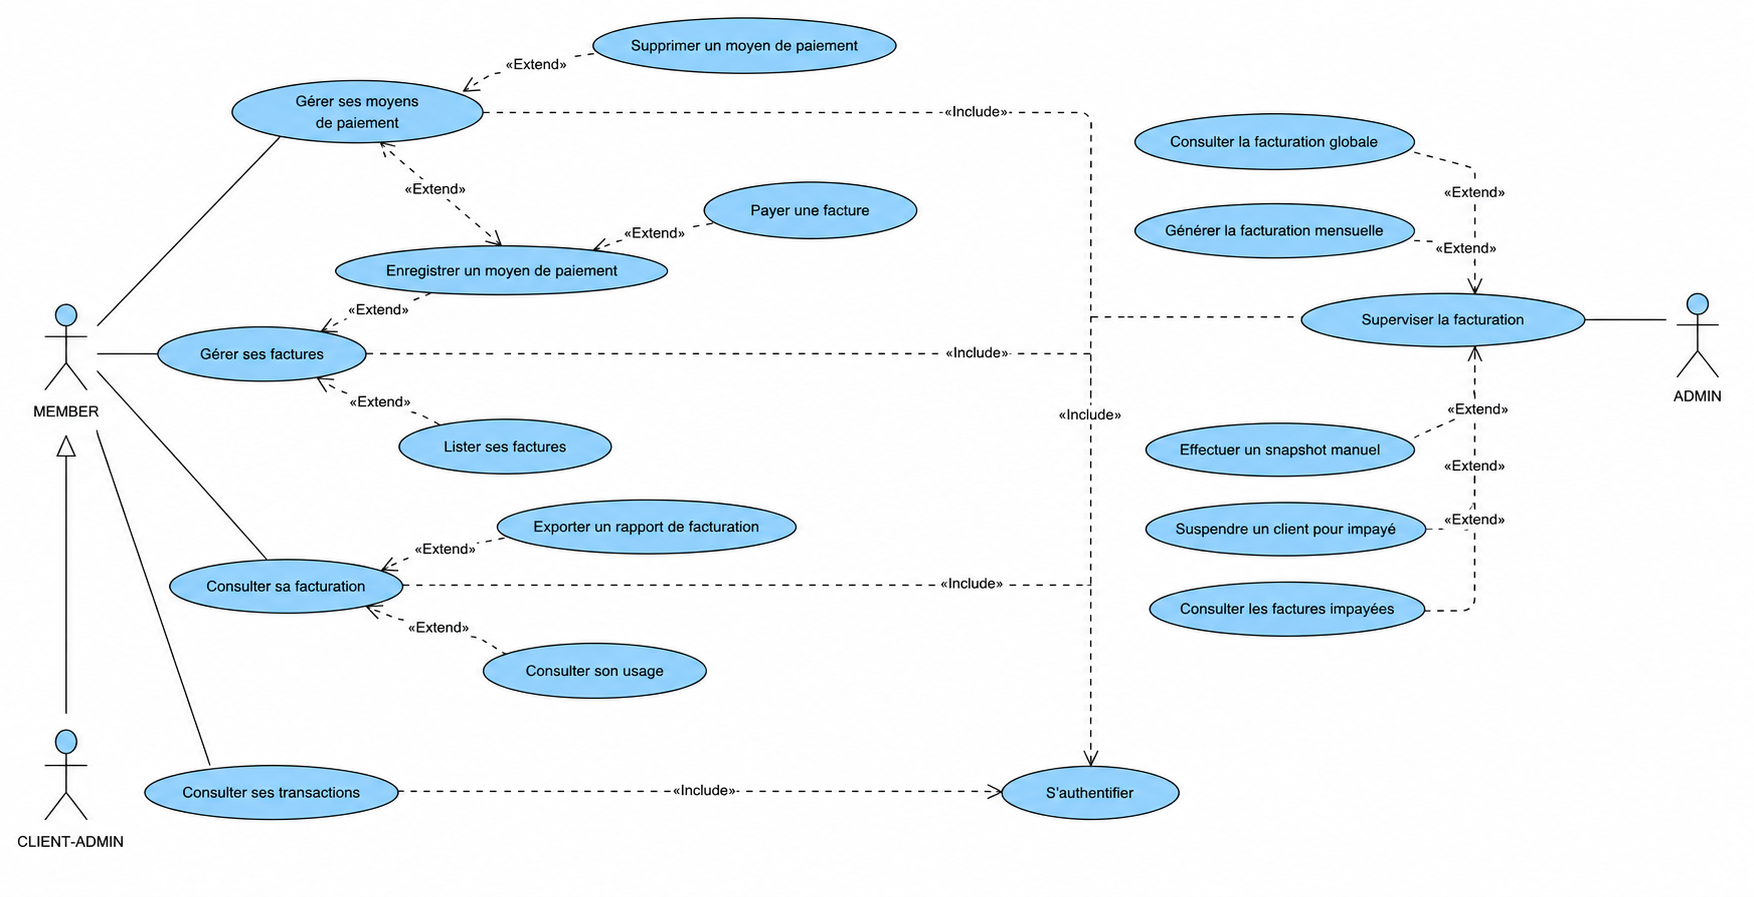
\includegraphics[width=\textwidth]{image/usescase7.png}
    \caption{Diagramme de cas d'utilisation du Sprint 7 — Gestion de la facturation et des paiements}
    \label{fig:uc-sprint7}
\end{figure}
\subsection{Services Web}
{\setlength{\tabcolsep}{8pt}
\begin{longtable}{|p{5.8cm}|p{8.4cm}|}
\hline
Service Web & Description \\
\hline
\endfirsthead
\hline
Service Web & Description \\
\hline
\endhead
\endfoot
\hline
\endlastfoot
\texttt{GET\slash api\slash billing\slash me} & Consulter sa facturation. \\ \hline
\texttt{GET\slash api\slash billing\slash export} & Exporter un rapport de facturation. \\ \hline
\texttt{GET\slash api\slash billing\slash admin} & Facturation globale, tous clients confondus (ADMIN). \\ \hline
\texttt{POST\slash api\slash billing\slash admin\slash snapshot} & Déclencher un instantané d'usage (ADMIN). \\ \hline
\texttt{GET\slash api\slash invoices} & Lister ses factures. \\ \hline
\texttt{POST\slash api\slash invoices\slash\{id\}\slash pay} & Payer une facture. \\ \hline
\texttt{GET\slash api\slash invoices\slash admin\slash overdue} & Factures impayées (ADMIN). \\ \hline
\texttt{POST\slash api\slash invoices\slash generate} & Générer les factures mensuelles (ADMIN). \\ \hline
\texttt{POST\slash api\slash invoices\slash apps\slash\{appId\}\slash suspend} & Suspendre une application pour impayé (ADMIN). \\ \hline
\texttt{GET\slash api\slash payment\slash config} & Configuration publique du prestataire de paiement. \\ \hline
\texttt{POST\slash api\slash payment\slash setup-intent} & Enregistrer un moyen de paiement. \\ \hline
\texttt{GET\slash api\slash payment\slash methods} & Lister ses moyens de paiement. \\ \hline
\texttt{DELETE\slash api\slash payment\slash methods\slash\{id\}} & Supprimer un moyen de paiement. \\ \hline
\texttt{POST\slash api\slash payment\slash pay} & Payer. \\ \hline
\texttt{GET\slash api\slash payment\slash transactions} & Historique des transactions. \\ \hline
\texttt{POST\slash api\slash payment\slash webhook} & Notification du prestataire de paiement. \\ \hline
\end{longtable}}

% \subsection{Services Web}

% \needspace{0.55\textheight}
% {\setlength{\tabcolsep}{8pt}
% \begin{longtable}{|p{5.8cm}|p{8.4cm}|}
% \hline
% Service Web & Description \\
% \hline
% \endfirsthead
% \hline
% Service Web & Description \\
% \hline
% \endhead
% \endfoot
% \hline
% \endlastfoot
% \texttt{GET /api/billing/me} & Consulter sa facturation. \\ \hline
% \texttt{GET /api/billing/export} & Exporter un rapport de facturation. \\ \hline
% \texttt{GET /api/billing/admin} & Facturation globale, tous clients confondus (ADMIN). \\ \hline
% \texttt{POST /api/billing/admin/snapshot} & Déclencher un instantané d'usage (ADMIN). \\ \hline
% \texttt{GET /api/invoices} & Lister ses factures. \\ \hline
% \texttt{POST /api/invoices/\{id\}/pay} & Payer une facture. \\ \hline
% \texttt{GET /api/invoices/admin/overdue} & Factures impayées (ADMIN). \\ \hline
% \texttt{POST /api/invoices/generate} & Générer les factures mensuelles (ADMIN). \\ \hline
% \texttt{POST /api/invoices/apps/\{appId\}/suspend} & Suspendre une application pour impayé (ADMIN). \\ \hline
% \texttt{GET /api/payment/config} & Configuration publique du prestataire de paiement. \\ \hline
% \texttt{POST /api/payment/setup-intent} & Enregistrer un moyen de paiement. \\ \hline
% \texttt{GET /api/payment/methods} & Lister ses moyens de paiement. \\ \hline
% \texttt{DELETE /api/payment/methods/\{id\}} & Supprimer un moyen de paiement. \\ \hline
% \texttt{POST /api/payment/pay} & Payer. \\ \hline
% \texttt{GET /api/payment/transactions} & Historique des transactions. \\ \hline
% \texttt{POST /api/payment/webhook} & Notification du prestataire de paiement. \\ \hline
% \end{longtable}}

\subsection{Conception}

Une fonctionnalité est détaillée : le paiement d'une facture, techniquement la plus riche puisqu'elle implique un prestataire externe.

\needspace{0.45\textheight}
\subsubsection{Cas d'utilisation : « Payer une facture »}

\subsubsection*{Description textuelle}

\renewcommand{\arraystretch}{1.5}
\begin{longtable}{|p{4cm}|p{11cm}|}
\hline
Nom & Payer une facture \\
\hline
Acteur & CLIENT\_ADMIN \\
\hline
Pré-condition & Un moyen de paiement est enregistré ; une facture est en attente de règlement \\
\hline
Scénario nominal & 1. Le CLIENT\_ADMIN sélectionne une facture en attente. 2. Le backend déclenche le règlement auprès du prestataire de paiement avec le moyen de paiement enregistré. 3. Le prestataire notifie le backend du résultat par webhook. 4. Le statut de la facture est mis à jour. \\
\hline
Post-condition & La facture est marquée réglée, ou l'échec est signalé à l'utilisateur. \\
\hline
\caption{Description textuelle du cas d'utilisation « Payer une facture »}
\label{tab:uc-pay}
\end{longtable}

\needspace{0.35\textheight}
\subsubsection*{Diagramme de séquence}

\begin{figure}[H]
 \centering
    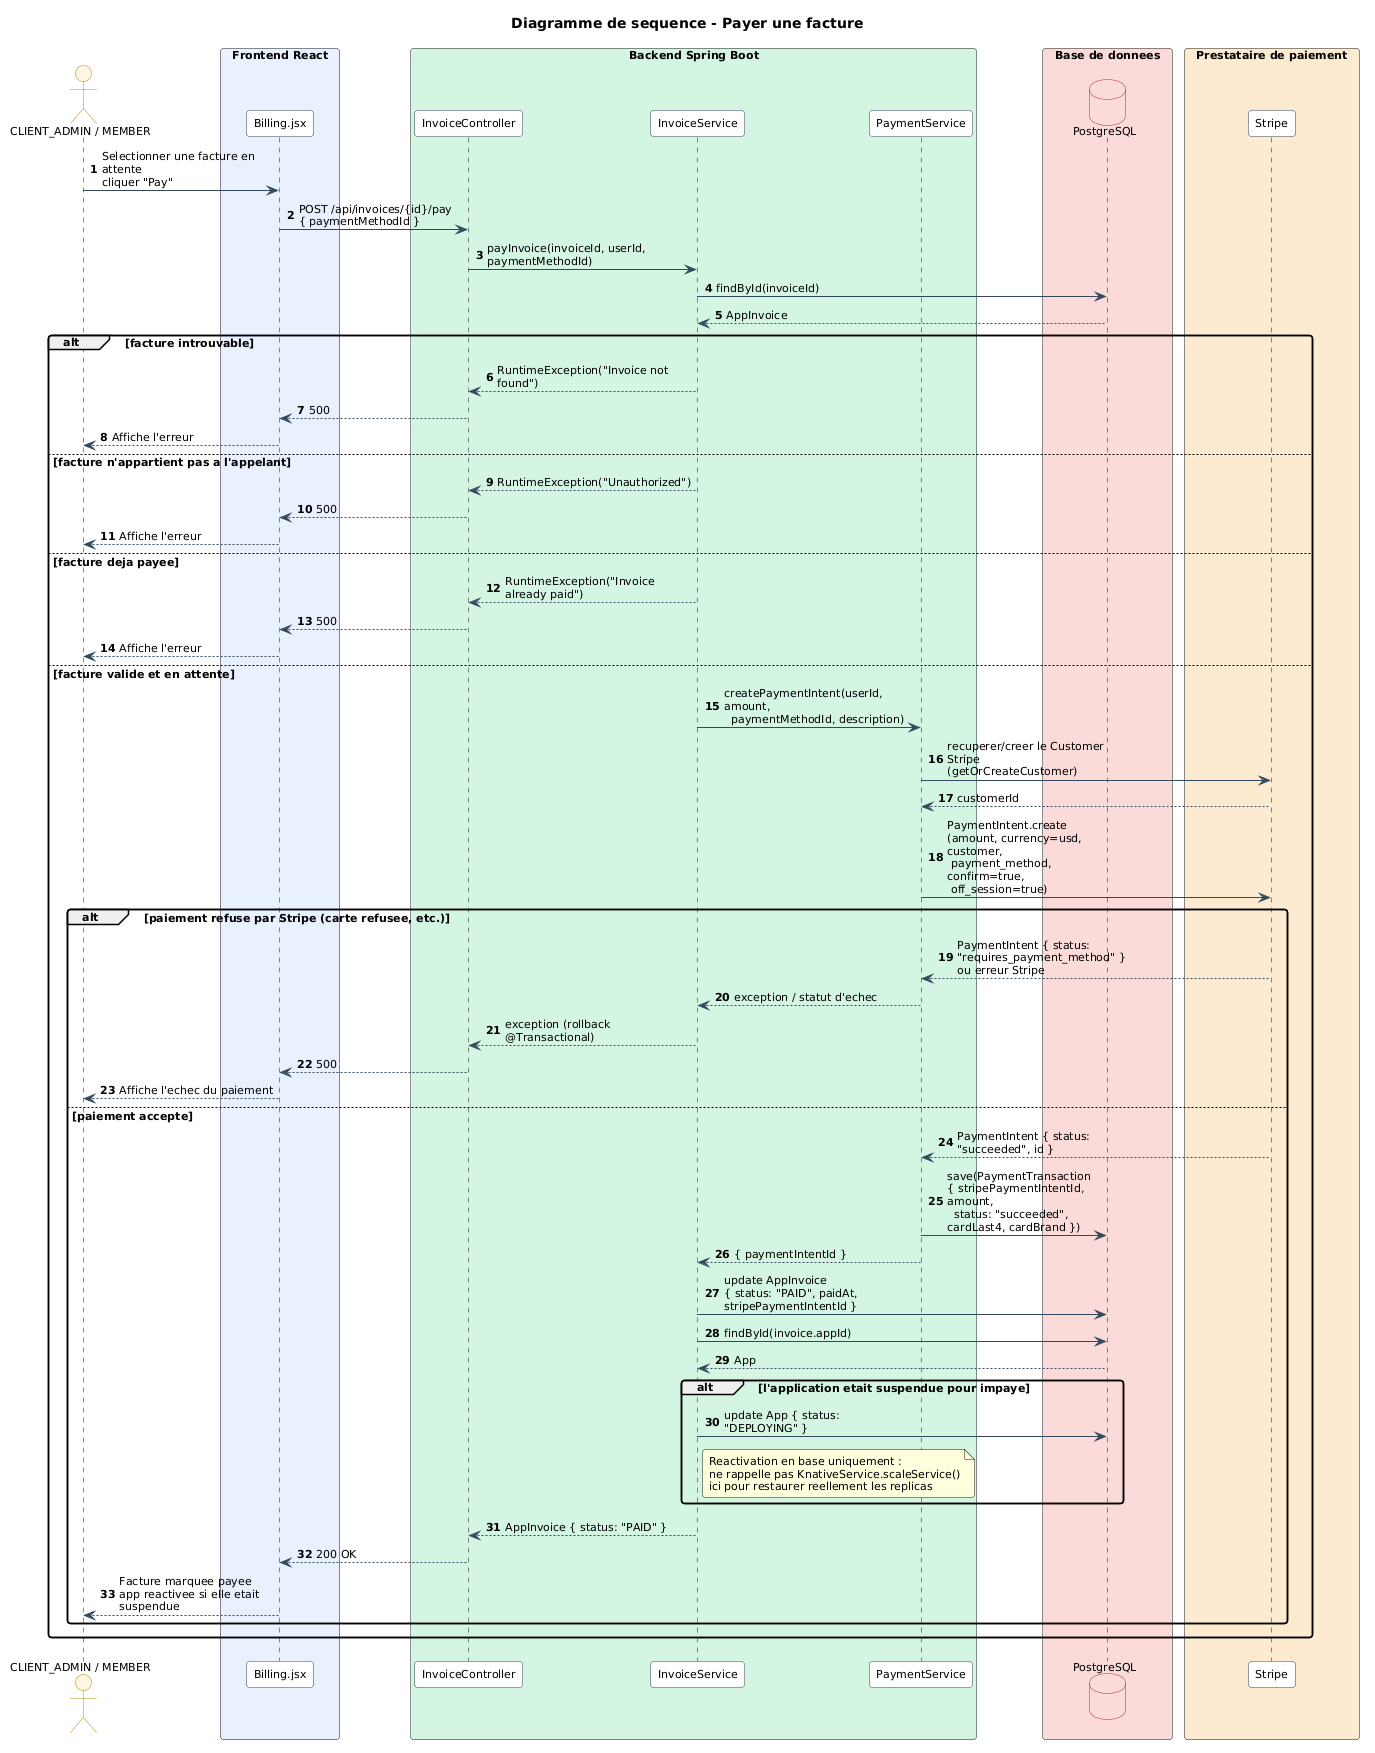
\includegraphics[width=0.9\textwidth]{image/seq-pay.png}
    \caption{Diagramme de séquence — Payer une facture}
    \label{fig:seq-pay}
\end{figure}

\subsection{Réalisation du Sprint 7}

Fonctionnalité : Consulter sa facturation, enregistrer un moyen de paiement et payer une facture. La page de facturation du portail regroupe, en un seul endroit, le coût projeté du mois en cours, l'historique des factures, les moyens de paiement enregistrés et l'historique des transactions.

\begin{figure}[H]
 \centering
    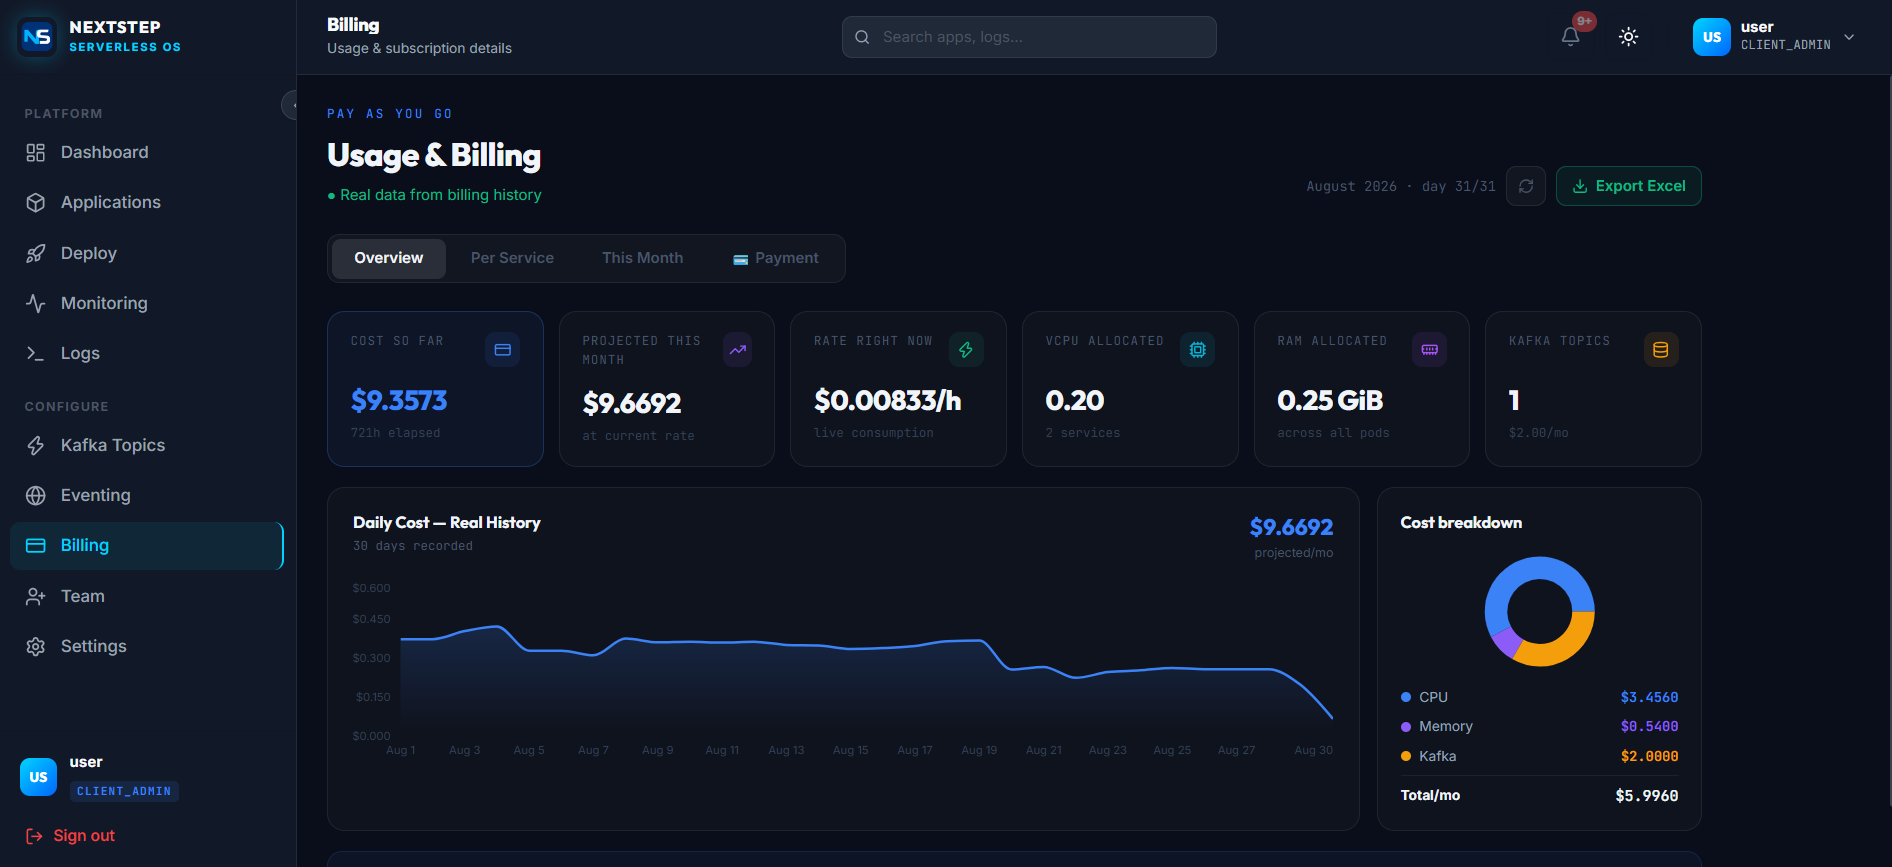
\includegraphics[width=0.9\textwidth]{image/Interface de facturation du compte client1.png}
    \caption{Interface de facturation du compte client}
    \label{fig:capture-billing}
\end{figure}

Fonctionnalité : Facturation globale et génération des factures (ADMIN). L'ADMIN consulte, depuis la console d'administration, la facturation de l'ensemble des clients et déclenche la génération des factures mensuelles.

\begin{figure}[H]
 \centering
    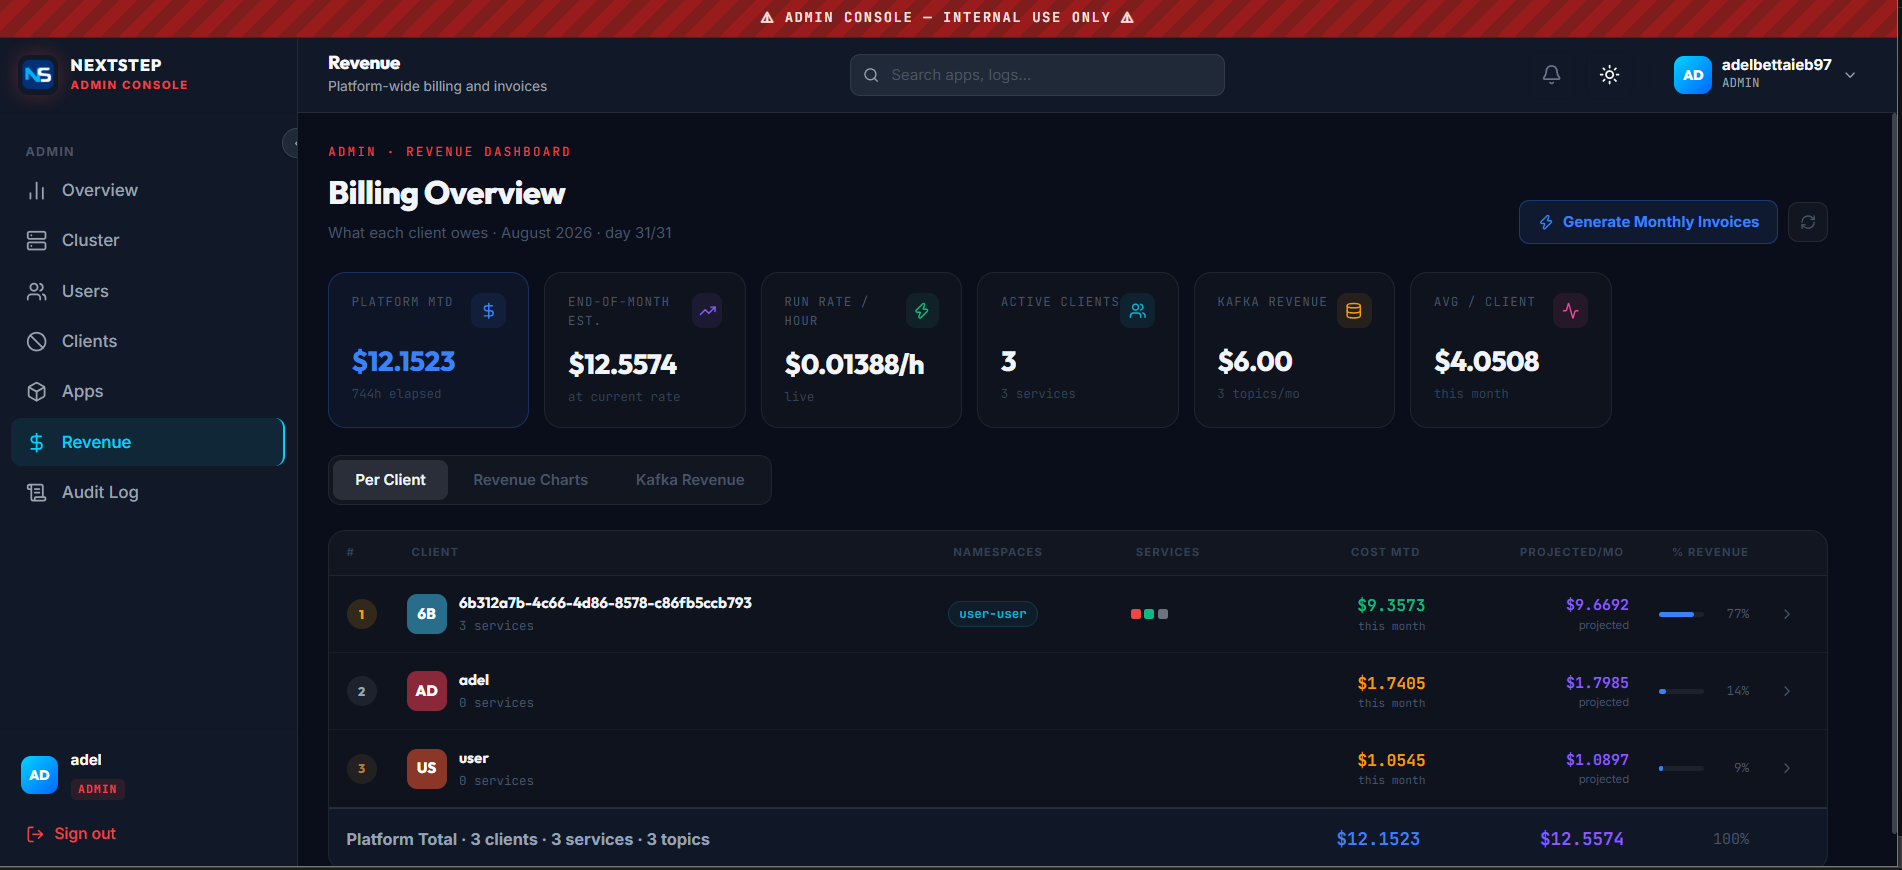
\includegraphics[width=0.9\textwidth]{image/Interface de facturation globale (console d’administration)1.png}
    \caption{Interface de facturation globale (console d'administration)}
    \label{fig:capture-adminbilling}
\end{figure}

Fonctionnalité : Payer une facture en retard (CLIENT\_ADMIN). Le client règle une facture en retard directement depuis l'onglet Payment de son portail, avec un moyen de paiement déjà enregistré.

\begin{figure}[H]
 \centering
    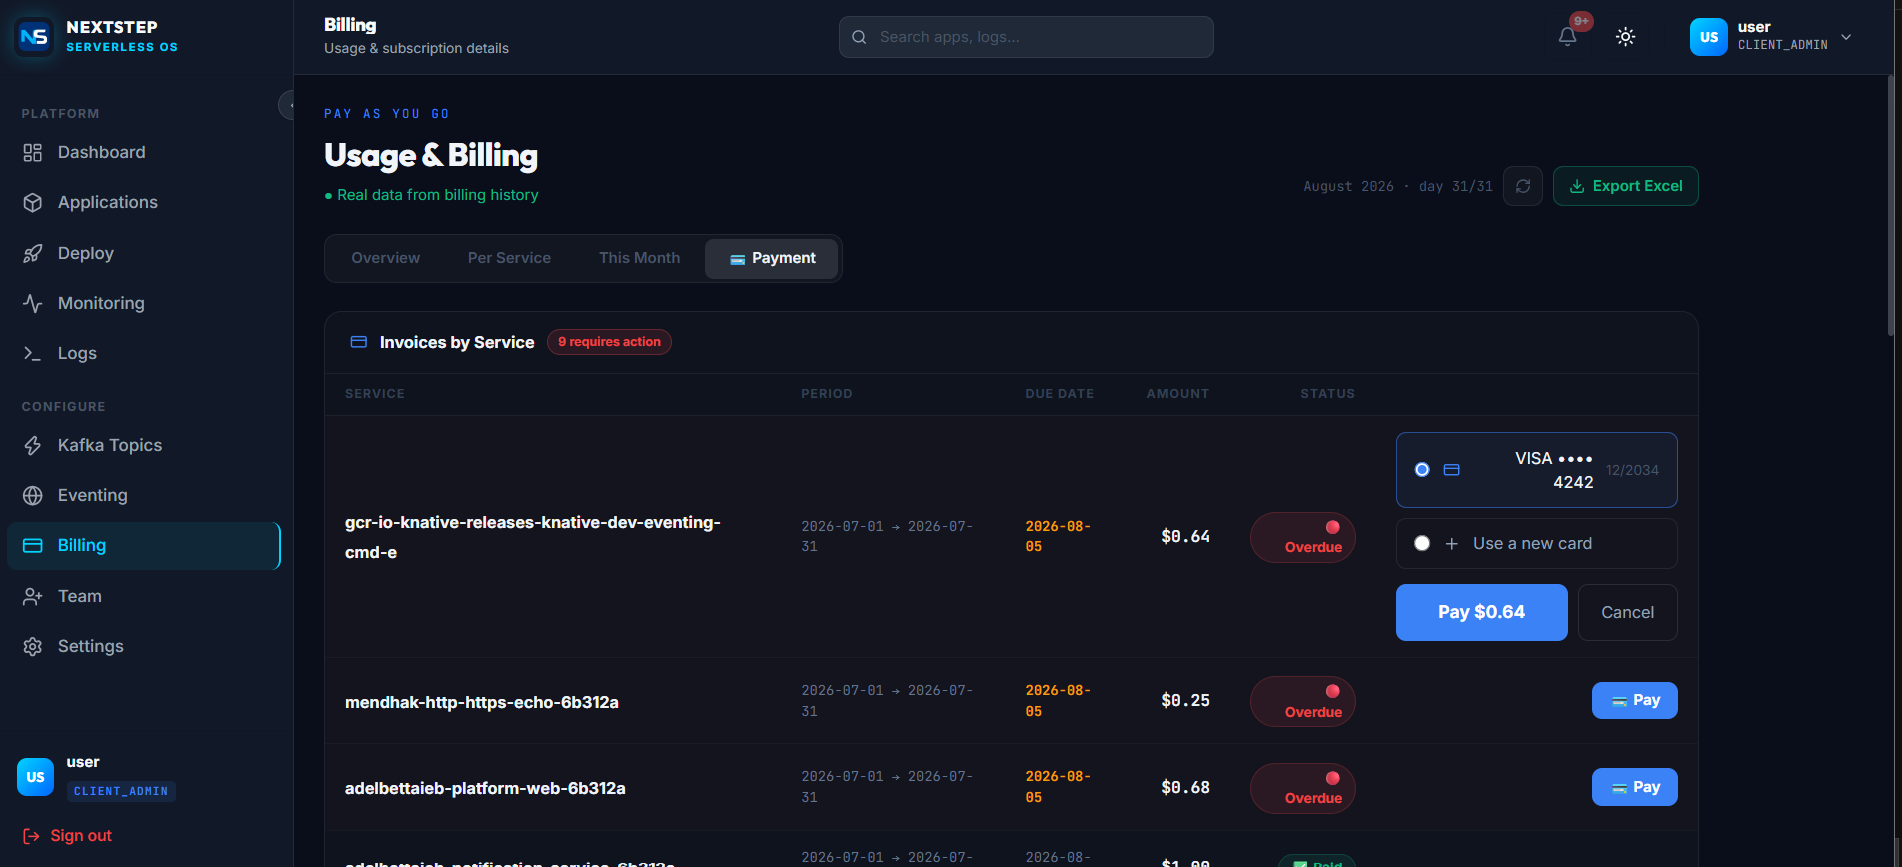
\includegraphics[width=0.9\textwidth]{image/payerune facture.png}
    \caption{Paiement d'une facture en retard par le client}
    \label{fig:capture-client-pay}
\end{figure}

\subsection{Conclusion}

Ce sprint livre la facturation à l'usage et son règlement en ligne, consultables par le client comme par l'équipe d'exploitation. Aucune limite de ressources par défaut n'est appliquée par tenant, ce qui expose le modèle à une facturation potentiellement illimitée en l'absence d'action du client ; ce point est repris au chapitre de validation.

\section{Sprint 8 : Gestion des comptes clients, des quotas et de l'audit}

\subsection{Introduction}

Ce sprint donne à l'ADMIN les moyens de gérer les comptes clients eux-mêmes : suspension, réactivation, quotas de ressources, et la traçabilité des actions administratives sensibles au travers d'un journal d'audit exportable. C'est un domaine exclusivement réservé à l'ADMIN, distinct de la gestion des utilisateurs individuels (Sprint 3).
\subsection{Sprint Backlog}
Le tableau~\ref{tab:sb-sprint8} présente le backlog détaillé du Sprint 8, obtenu en décomposant chaque User Story retenue en tâches techniques.

{
\setlength{\LTleft}{-1.5cm}
\setlength{\LTright}{-1.5cm}
\setlength{\tabcolsep}{8pt}
\renewcommand{\arraystretch}{1.9}
\begin{longtable}{|p{6.6cm}|>{\raggedright\arraybackslash}p{8.1cm}|>{\centering\arraybackslash}p{2.3cm}|}
\hline
User Story & Tâches & Estimation \\
\hline
\endfirsthead

\multicolumn{3}{l}{\small\itshape (suite du tableau~\ref{tab:sb-sprint8})}\\
\hline
User Story & Tâches & Estimation \\
\hline
\endhead

\hline
\multicolumn{3}{r}{\small\itshape (suite page suivante)}\\
\endfoot

\hline
\caption{Backlog du Sprint 8}
\label{tab:sb-sprint8}
\endlastfoot

\multirow{4}{6.6cm}{\centering En tant qu'ADMIN, je veux lister et suspendre ou réactiver un compte client afin de gérer les abus ou les impayés.}
& Développer la liste des comptes clients avec leur état. & 1 \\* \cline{2-3}
& Développer la suspension d'un compte. & 2 \\* \cline{2-3}
& Développer la réactivation d'un compte. & 1 \\* \cline{2-3}
& Tester ces actions. & 1 \\ \hline

\multirow{3}{6.6cm}{\centering En tant qu'ADMIN, je veux consulter et modifier le quota de ressources d'un client afin d'encadrer sa consommation.}
& Développer la consultation du quota. & 1 \\* \cline{2-3}
& Développer la modification du quota. & 1 \\* \cline{2-3}
& Propager le quota vers le cluster. & 2 \\ \hline

\multirow{3}{6.6cm}{\centering En tant qu'ADMIN, je veux consulter et exporter le journal d'audit des actions administratives afin de garder une traçabilité.}
& Développer l'enregistrement automatique des actions administratives. & 2 \\* \cline{2-3}
& Développer la consultation paginée et filtrable du journal. & 2 \\* \cline{2-3}
& Développer l'export CSV. & 1 \\ \hline
\end{longtable}
}

% \subsection{Sprint Backlog}

% Le tableau~\ref{tab:sb-sprint8} présente le backlog détaillé du Sprint 8, obtenu en décomposant chaque User Story retenue en tâches techniques.

% \needspace{0.75\textheight}
% {
% \setlength{\LTleft}{-1.5cm}
% \setlength{\LTright}{-1.5cm}
% \setlength{\tabcolsep}{8pt}
% \renewcommand{\arraystretch}{1.9}
% \begin{longtable}{|p{6.6cm}|>{\raggedright\arraybackslash}p{8.1cm}|>{\centering\arraybackslash}p{2.3cm}|}
% \hline
% User Story & Tâches & Estimation \\
% \hline
% \endfirsthead
% \hline
% User Story & Tâches & Estimation \\
% \hline
% \endhead
% \endfoot
% \hline

% \caption{Backlog du Sprint 8}
% \label{tab:sb-sprint8}
% \endlastfoot

% \multirow{4}{6.6cm}{\centering En tant qu'ADMIN, je veux lister et suspendre ou réactiver un compte client afin de gérer les abus ou les impayés.}
% & Développer la liste des comptes clients avec leur état. & 1 \\ \cline{2-3}
% & Développer la suspension d'un compte. & 1 \\ \cline{2-3}
% & Développer la réactivation d'un compte. & 1 \\ \cline{2-3}
% & Tester ces actions. & 1 \\ \hline

% \multirow{3}{6.6cm}{\centering En tant qu'ADMIN, je veux consulter et modifier le quota de ressources d'un client afin d'encadrer sa consommation.}
% & Développer la consultation du quota. & 1 \\ \cline{2-3}
% & Développer la modification du quota. & 1 \\ \cline{2-3}
% & Propager le quota vers le cluster. & 1 \\ \hline

% \multirow{3}{6.6cm}{\centering En tant qu'ADMIN, je veux consulter et exporter le journal d'audit des actions administratives afin de garder une traçabilité.}
% & Développer l'enregistrement automatique des actions administratives. & 1 \\ \cline{2-3}
% & Développer la consultation paginée et filtrable du journal. & 1 \\ \cline{2-3}
% & Développer l'export CSV. & 1 \\ \hline

% \end{longtable}
% }

\subsection{Diagramme de cas d'utilisation du Sprint 8}

Acteur unique : ADMIN. Le diagramme réunit l'ensemble des fonctionnalités du sprint : gestion des comptes clients, gestion des quotas, consultation et export du journal d'audit.

\begin{figure}[H]
 \centering
    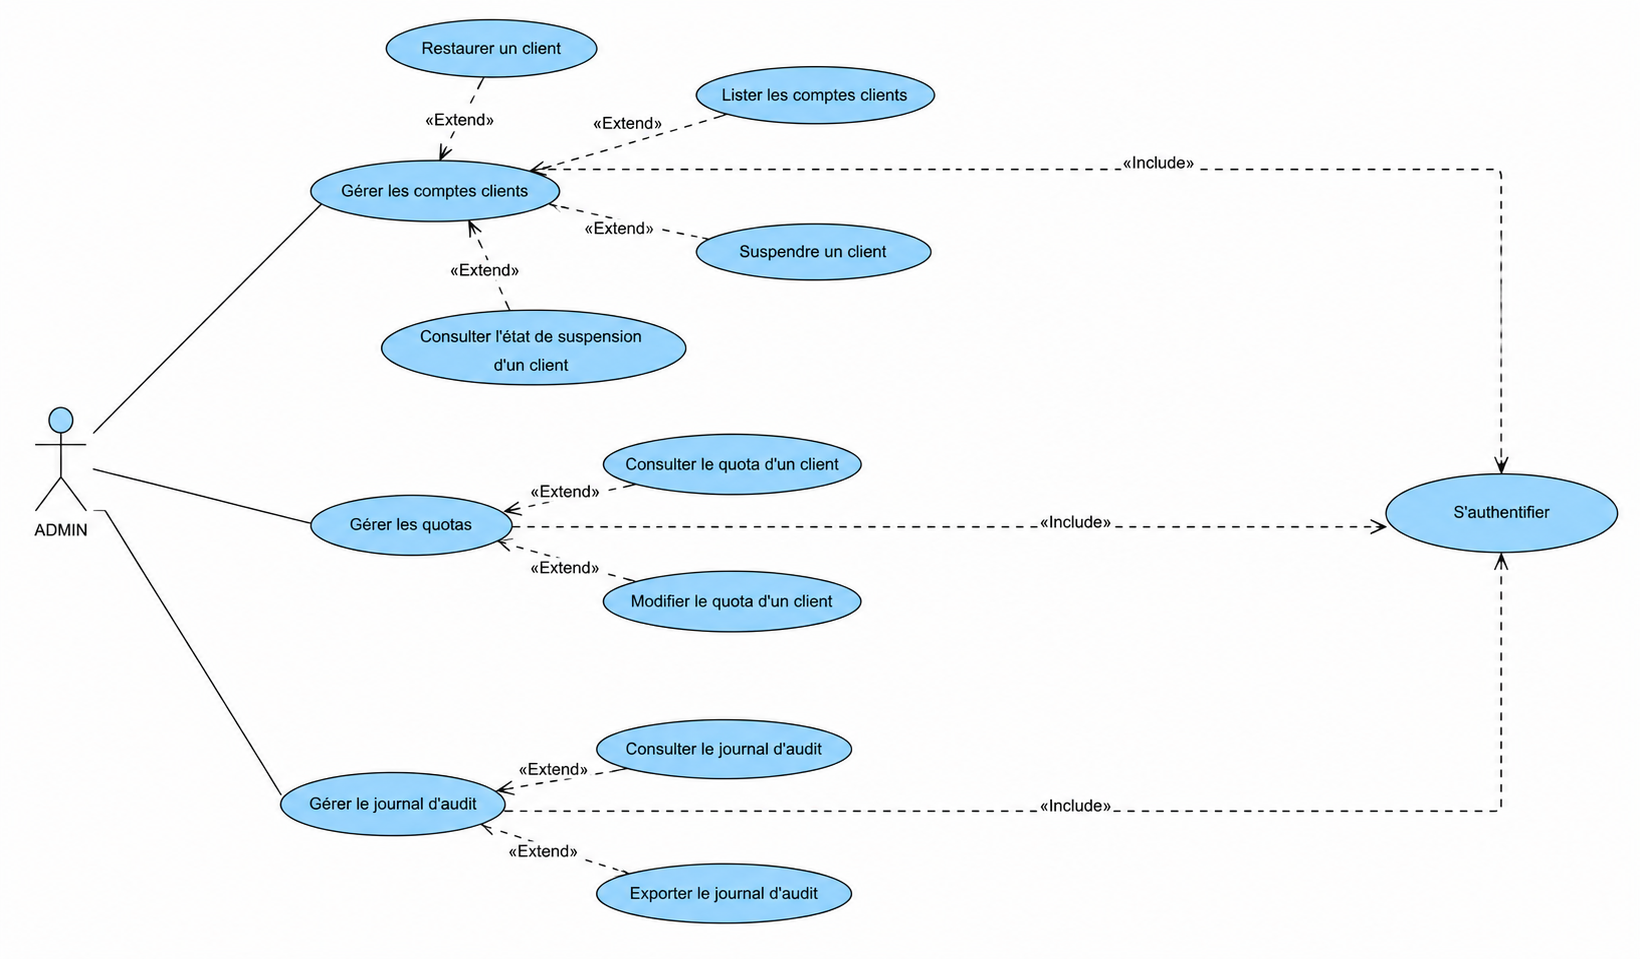
\includegraphics[width=\textwidth]{image/ucsprint8.png}
    \caption{Diagramme de cas d'utilisation du Sprint 8 — Comptes clients, quotas et audit}
    \label{fig:uc-sprint8}
\end{figure}
\subsection{Services Web}
{\setlength{\tabcolsep}{8pt}
\begin{longtable}{|p{5.8cm}|p{8.4cm}|}
\hline
Service Web & Description \\
\hline
\endfirsthead
\hline
Service Web & Description \\
\hline
\endhead
\endfoot
\hline
\endlastfoot
\texttt{GET\slash api\slash admin\slash clients} & Lister les comptes clients avec leur état de suspension. \\ \hline
\texttt{POST\slash api\slash admin\slash clients\slash\{userId\}\slash suspend} & Suspendre un compte client. \\ \hline
\texttt{POST\slash api\slash admin\slash clients\slash\{userId\}\slash restore} & Réactiver un compte client. \\ \hline
\texttt{GET\slash api\slash admin\slash clients\slash\{userId\}\slash quota} & Consulter le quota d'un client. \\ \hline
\texttt{PUT\slash api\slash admin\slash clients\slash\{userId\}\slash quota} & Modifier le quota d'un client. \\ \hline
\texttt{GET\slash api\slash admin\slash audit-log} & Consulter le journal d'audit, paginé et filtrable. \\ \hline
\texttt{GET\slash api\slash admin\slash audit-log\slash export} & Exporter le journal d'audit (CSV). \\ \hline
\end{longtable}}
% \subsection{Services Web}

% \needspace{0.55\textheight}
% {\setlength{\tabcolsep}{8pt}
% \begin{longtable}{|p{5.8cm}|p{8.4cm}|}
% \hline
% Service Web & Description \\
% \hline
% \endfirsthead
% \hline
% Service Web & Description \\
% \hline
% \endhead
% \endfoot
% \hline
% \endlastfoot
% \texttt{GET /api/admin/clients} & Lister les comptes clients avec leur état de suspension. \\ \hline
% \texttt{POST /api/admin/clients/\{userId\}/suspend} & Suspendre un compte client. \\ \hline
% \texttt{POST /api/admin/clients/\{userId\}/restore} & Réactiver un compte client. \\ \hline
% \texttt{GET /api/admin/clients/\{userId\}/quota} & Consulter le quota d'un client. \\ \hline
% \texttt{PUT /api/admin/clients/\{userId\}/quota} & Modifier le quota d'un client. \\ \hline
% \texttt{GET /api/admin/audit-log} & Consulter le journal d'audit, paginé et filtrable. \\ \hline
% \texttt{GET /api/admin/audit-log/export} & Exporter le journal d'audit (CSV). \\ \hline
% \end{longtable}}

\subsection{Conception}

Deux fonctionnalités sont détaillées : la suspension d'un compte client, l'action de gouvernance la plus significative de ce sprint ; la consultation du journal d'audit, qui trace précisément ce type d'action.

\needspace{0.45\textheight}
\subsubsection{Cas d'utilisation : « Suspendre un compte client »}

\subsubsection*{Description textuelle}

\renewcommand{\arraystretch}{1.5}
\begin{longtable}{|p{4cm}|p{11cm}|}
\hline
Nom & Suspendre un compte client \\
\hline
Acteur & ADMIN \\
\hline
Pré-condition & Le compte client existe et n'est pas déjà suspendu \\
\hline
Scénario nominal & 1. L'ADMIN sélectionne un compte client depuis la console d'administration. 2. Il déclenche la suspension. 3. Le backend suspend l'ensemble des services du client. 4. L'action est journalisée dans le journal d'audit. \\
\hline
Post-condition & Les services du client sont suspendus, l'action est tracée. \\
\hline
\caption{Description textuelle du cas d'utilisation « Suspendre un compte client »}
\label{tab:uc-suspend-client}
\end{longtable}

\needspace{0.35\textheight}
\subsubsection*{Diagramme de séquence}

\begin{figure}[H]
 \centering
    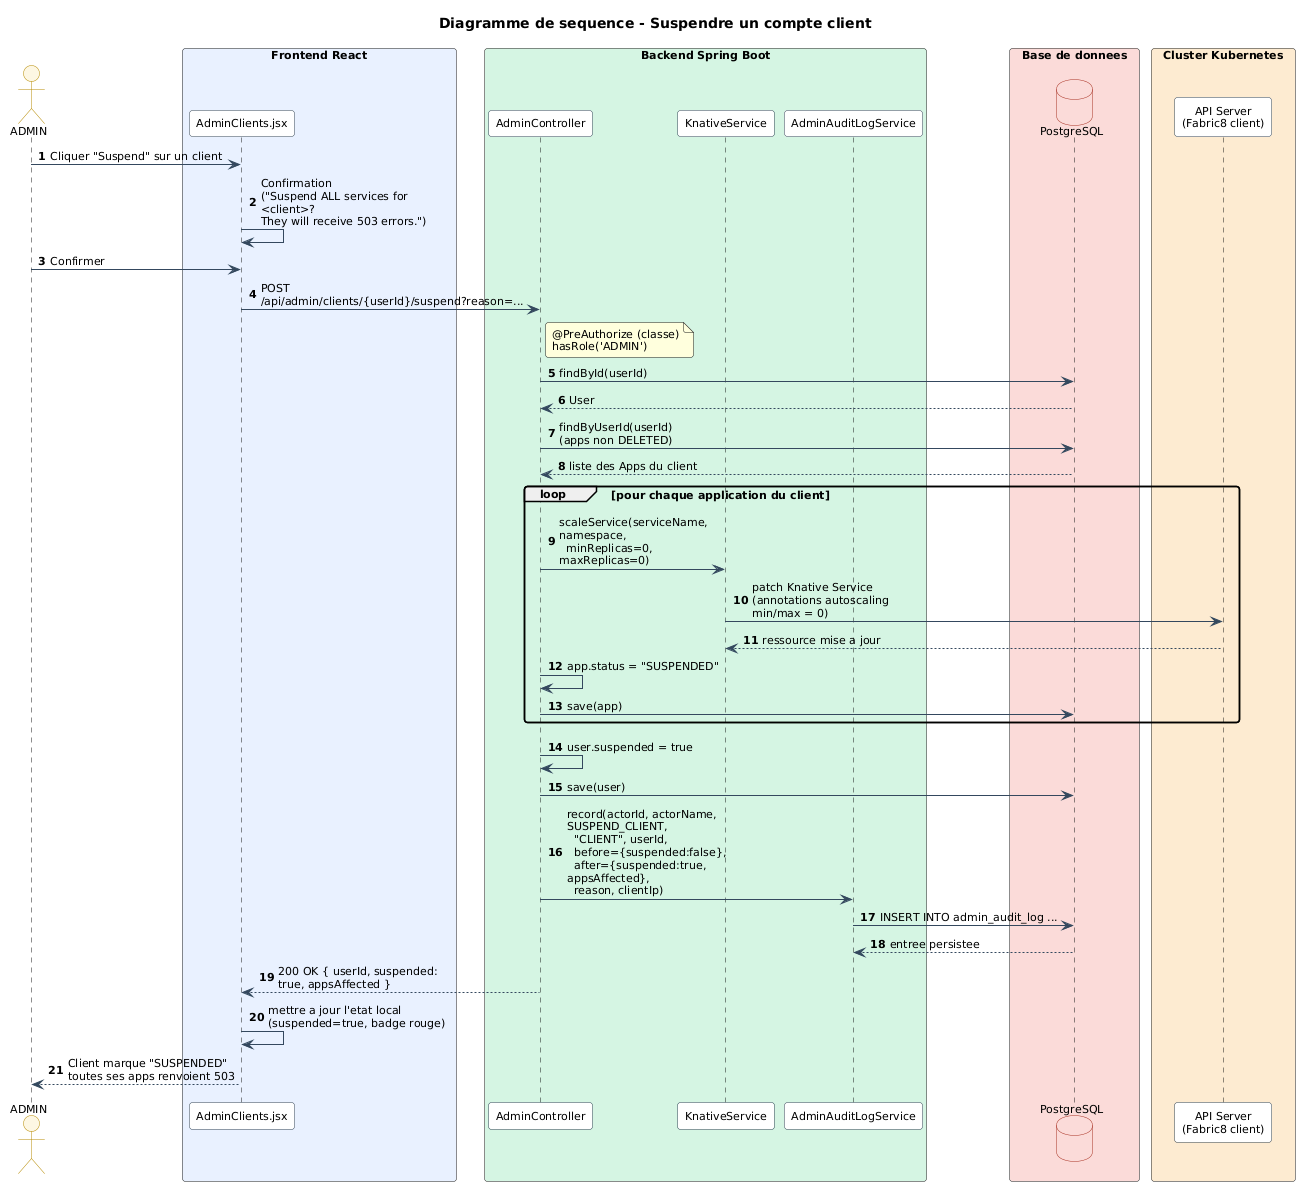
\includegraphics[width=0.9\textwidth]{image/secanse8suspendeapp.png}
    \caption{Diagramme de séquence — Suspendre un compte client}
    \label{fig:seq-suspend}
\end{figure}

\subsection{Réalisation du Sprint 8}

Fonctionnalité : Gérer les comptes clients — suspension, réactivation et quotas. La console d'administration liste les comptes clients avec leur état, permet de les suspendre ou de les réactiver, et de consulter/modifier leur quota de ressources (CPU, mémoire, nombre maximal d'applications), propagé au cluster.

\begin{figure}[H]
 \centering
    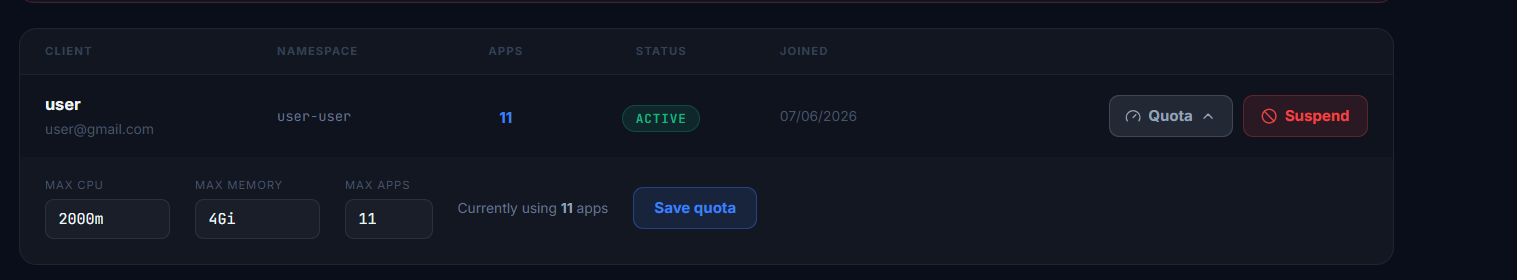
\includegraphics[width=0.9\textwidth]{image/Interface de gestion des quotas .png}
    \caption{Gestion des comptes clients}
    \label{fig:capture-quota}
\end{figure}

Fonctionnalité : Consulter et exporter le journal d'audit. Le journal d'audit liste les actions administratives sensibles, filtrables et exportables.

\begin{figure}[H]
 \centering
    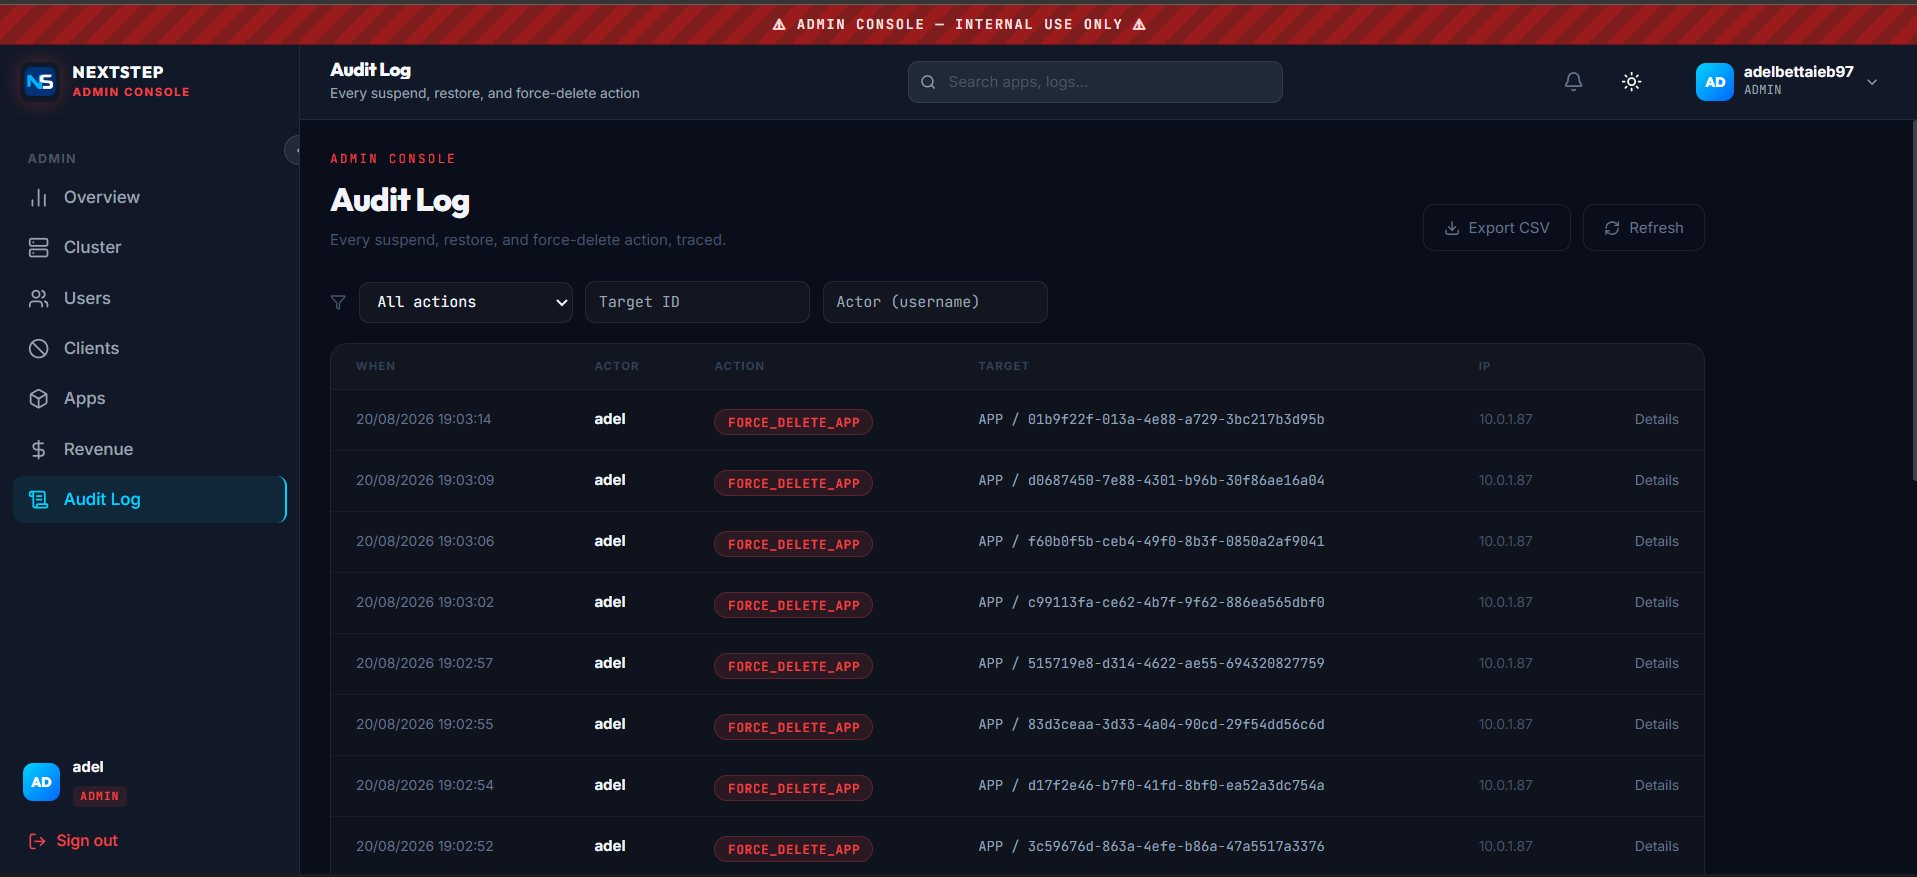
\includegraphics[width=0.9\textwidth]{image/Interface du journal d'audit.png}
    \caption{Interface du journal d'audit}
    \label{fig:capture-auditlog}
\end{figure}

Les actions tracées sont limitées à huit types : suspension et réactivation d'un compte client, suspension, réactivation, suppression forcée et redimensionnement d'une application, suppression forcée d'un sujet Kafka, et modification d'un quota. Le journal d'audit ne trace donc que la gouvernance administrative, jamais les consultations.

\subsection{Conclusion}

Ce sprint donne à l'ADMIN les leviers de gouvernance des comptes clients, avec une traçabilité systématique de leur usage. Il complète, sur le plan administratif, ce que le Sprint 9 complète sur le plan de la supervision technique du cluster.


\section{Sprint 9 : Gestion de l'exploitation du cluster et du statut public}

\subsection{Introduction}

Ce sprint dote l'ADMIN d'une supervision complète de l'état du cluster Kubernetes, et expose au public une page de statut synthétique de la disponibilité de la plateforme. Les deux fonctionnalités s'appuient sur la même donnée de santé du cluster, l'une en détail et en interne, l'autre de façon synthétique et publique.

\subsection{Sprint Backlog}

Le tableau~\ref{tab:sb-sprint9} présente le backlog détaillé du Sprint 9, obtenu en décomposant chaque User Story retenue en tâches techniques.

{
\setlength{\LTleft}{-1.5cm}
\setlength{\LTright}{-1.5cm}
\setlength{\tabcolsep}{8pt}
\renewcommand{\arraystretch}{1.9}
\begin{longtable}{|p{6.6cm}|>{\raggedright\arraybackslash}p{8.1cm}|>{\centering\arraybackslash}p{2.3cm}|}
\hline
User Story & Tâches & Estimation \\
\hline
\endfirsthead
\hline
User Story & Tâches & Estimation \\
\hline
\endhead
\endfoot
\hline

\caption{Backlog du Sprint 9}
\label{tab:sb-sprint9}
\endlastfoot

\multirow{3}{6.6cm}{\centering En tant qu'ADMIN, je veux consulter l'état complet du cluster Kubernetes afin de superviser l'infrastructure.}
& Développer la consultation des nœuds, pods, namespaces et volumes. & 2 \\ \cline{2-3}
& Développer la consultation des services Knative et des courtiers Kafka. & 2 \\ \cline{2-3}
& Développer la vue d'ensemble consolidée du cluster. & 2 \\ \hline

\multirow{3}{6.6cm}{\centering En tant qu'ADMIN, je veux consulter les alertes et les événements du cluster afin de détecter rapidement les incidents.}
& Développer la consultation des alertes actives. & 1 \\ \cline{2-3}
& Développer la consultation des événements d'avertissement récents. & 1 \\ \cline{2-3}
& Développer la santé des composants système. & 1 \\ \hline

\end{longtable}
}

\subsection{Diagramme de cas d'utilisation du Sprint 9}

Le diagramme réunit l'ADMIN (supervision détaillée du cluster) et le Public non authentifié (statut synthétique), ce dernier accès restant également ouvert aux trois autres rôles une fois connectés.

\begin{figure}[H]
 \centering
    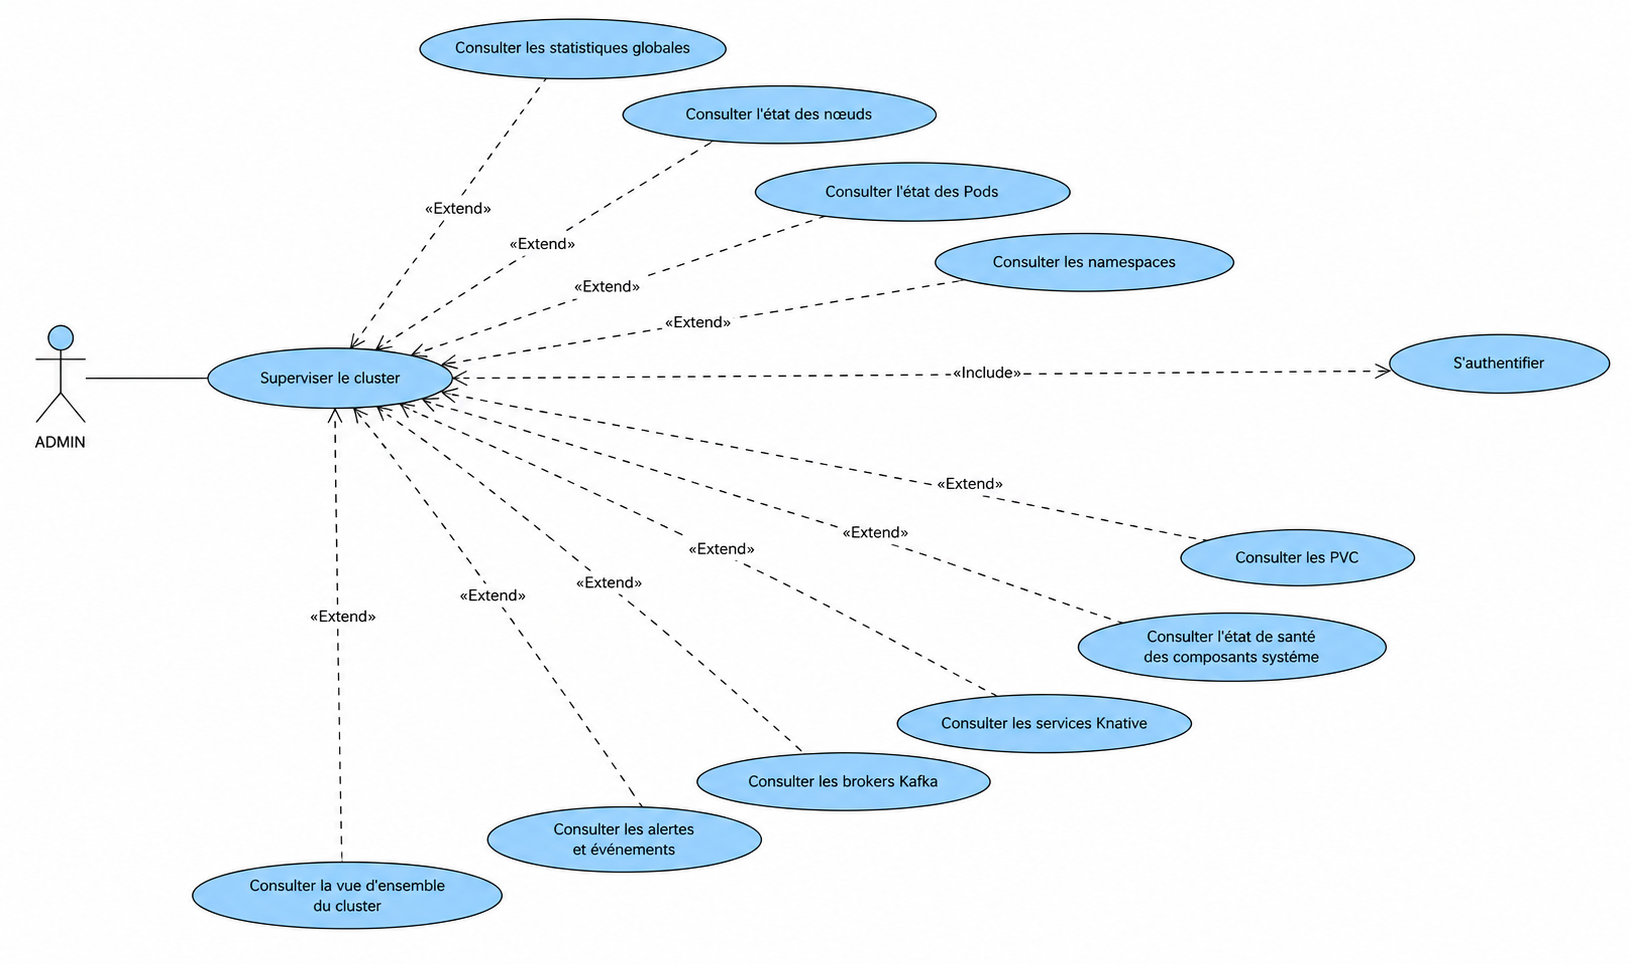
\includegraphics[width=\textwidth]{image/uc9.png}
    \caption{Diagramme de cas d'utilisation du Sprint 9 — Exploitation du cluster et statut public}
    \label{fig:uc-sprint9}
\end{figure}
\subsection{Services Web}
{\setlength{\tabcolsep}{8pt}
\begin{longtable}{|p{5.8cm}|p{8.4cm}|}
\hline
Service Web & Description \\
\hline
\endfirsthead
\hline
Service Web & Description \\
\hline
\endhead
\endfoot
\hline
\endlastfoot
\texttt{GET\slash api\slash admin\slash stats} & Statistiques globales de la plateforme (ADMIN). \\ \hline
\texttt{GET\slash api\slash admin\slash cluster\slash nodes}, \texttt{\slash namespaces}, \texttt{\slash pods}, \texttt{\slash storage} & État des nœuds, espaces de noms, pods et volumes (ADMIN). \\ \hline
\texttt{GET\slash api\slash admin\slash cluster\slash knative\slash services}, \texttt{\slash kafka\slash brokers} & État des services Knative et des courtiers Kafka (ADMIN). \\ \hline
\texttt{GET\slash api\slash admin\slash cluster\slash alerts}, \texttt{\slash events} & Alertes actives et événements d'avertissement récents (ADMIN). \\ \hline
\texttt{GET\slash api\slash admin\slash cluster\slash system-components} & Santé des composants système (ADMIN). \\ \hline
\texttt{GET\slash api\slash admin\slash cluster\slash overview} & Vue d'ensemble consolidée du cluster (ADMIN). \\ \hline
\texttt{GET\slash api\slash metrics\slash cluster} & Métriques agrégées du cluster (ADMIN). \\ \hline
\end{longtable}}
% \subsection{Services Web}

% \needspace{0.55\textheight}
% {\setlength{\tabcolsep}{8pt}
% \begin{longtable}{|p{5.8cm}|p{8.4cm}|}
% \hline
% Service Web & Description \\
% \hline
% \endfirsthead
% \hline
% Service Web & Description \\
% \hline
% \endhead
% \endfoot
% \hline
% \endlastfoot
% \texttt{GET /api/admin/stats} & Statistiques globales de la plateforme (ADMIN). \\ \hline
% \texttt{GET /api/admin/cluster/nodes}, \texttt{/namespaces}, \texttt{/pods}, \texttt{/storage} & État des nœuds, espaces de noms, pods et volumes (ADMIN). \\ \hline
% \texttt{GET /api/admin/cluster/knative/services}, \texttt{/kafka/brokers} & État des services Knative et des courtiers Kafka (ADMIN). \\ \hline
% \texttt{GET /api/admin/cluster/alerts}, \texttt{/events} & Alertes actives et événements d'avertissement récents (ADMIN). \\ \hline
% \texttt{GET /api/admin/cluster/system-components} & Santé des composants système (ADMIN). \\ \hline
% \texttt{GET /api/admin/cluster/overview} & Vue d'ensemble consolidée du cluster (ADMIN). \\ \hline
% \texttt{GET /api/metrics/cluster} & Métriques agrégées du cluster (ADMIN). \\ \hline
% \end{longtable}}

\subsection{Conception}

Deux fonctionnalités sont détaillées : la supervision du cluster, cœur du sprint côté ADMIN ; le statut public, fonctionnalité livrée dans le code mais jusqu'ici absente de ce mémoire.

\needspace{0.45\textheight}
\subsubsection{Cas d'utilisation : « Superviser le cluster »}

\subsubsection*{Description textuelle}

\renewcommand{\arraystretch}{1.5}
\begin{longtable}{|p{4cm}|p{11cm}|}
\hline
Nom & Superviser le cluster \\
\hline
Acteur & ADMIN \\
\hline
Pré-condition & L'ADMIN est authentifié sur la console d'administration \\
\hline
Scénario nominal & 1. L'ADMIN ouvre la page de supervision du cluster. 2. Le backend consulte l'API Kubernetes (nœuds, pods, espaces de noms) et Alertmanager (alertes actives). 3. L'état du cluster et les alertes actives sont affichés. \\
\hline
Post-condition & L'ADMIN dispose d'une vue à jour de l'état global du cluster. \\
\hline
\caption{Description textuelle du cas d'utilisation « Superviser le cluster »}
\label{tab:uc-cluster}
\end{longtable}

\needspace{0.35\textheight}
\subsubsection*{Diagramme de séquence}


\begin{figure}[H]
 \centering
    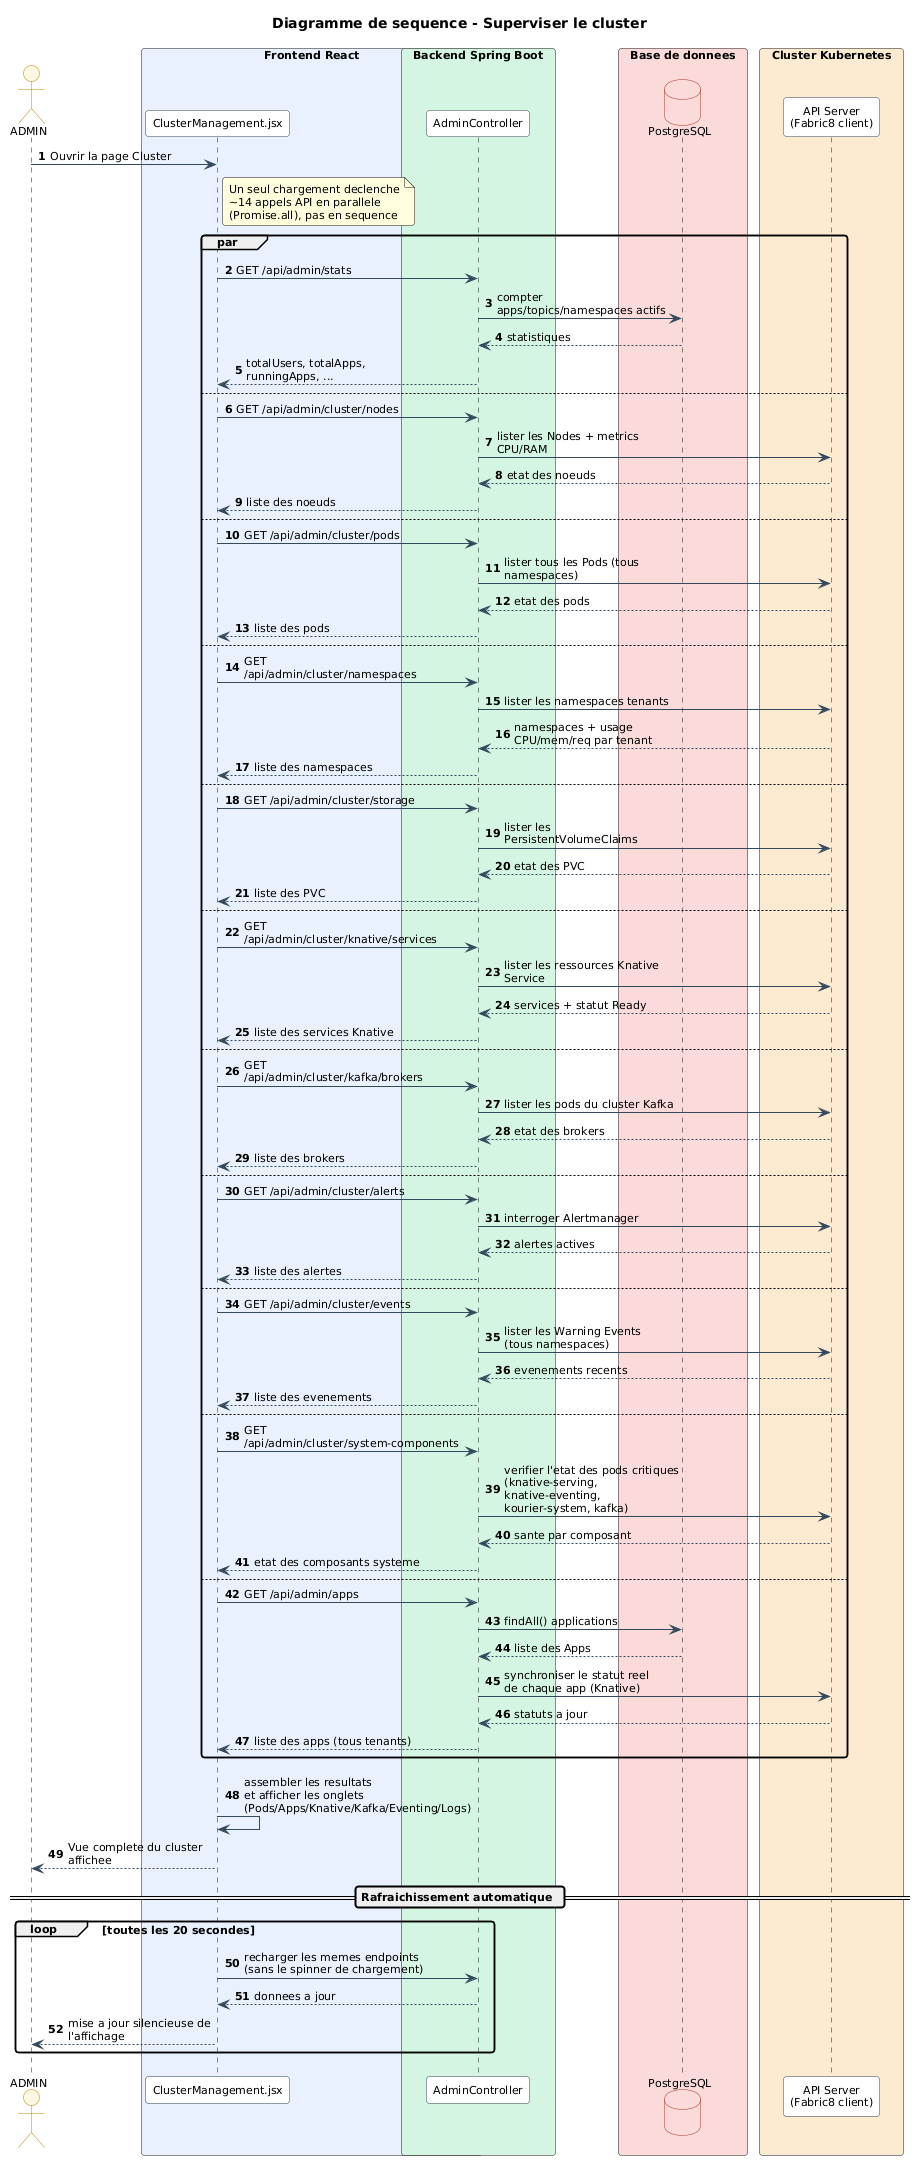
\includegraphics[width=0.9\textwidth]{image/seq-cluster.png}
    \caption{Diagramme de séquence — Superviser le cluster}
    \label{fig:seq-cluster}
\end{figure}

\subsection{Réalisation du Sprint 9}

Fonctionnalité : Superviser le cluster. La console d'administration affiche l'état des nœuds, des pods et des alertes actives du cluster.

\begin{figure}[H]
 \centering
    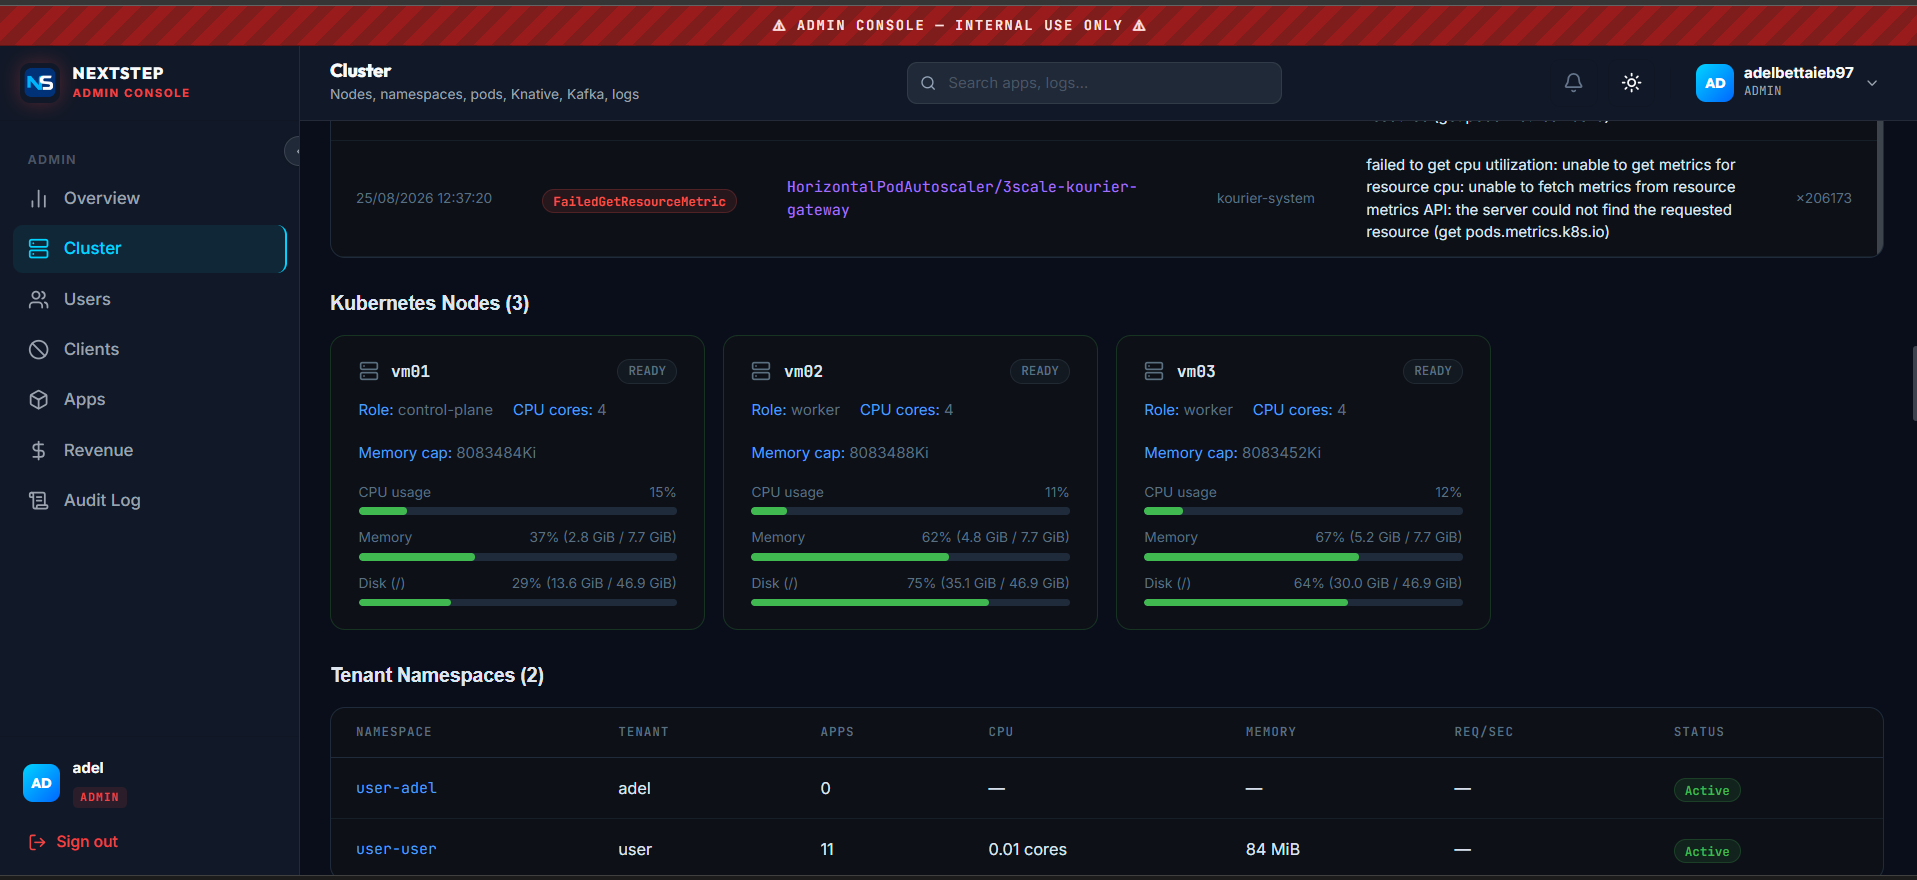
\includegraphics[width=0.9\textwidth]{image/Interface de supervision du cluster.png}
    \caption{Interface de supervision du cluster}
    \label{fig:capture-cluster}
\end{figure}

Fonctionnalité : Consulter les alertes et événements du cluster. Les alertes Alertmanager actives et les événements d'avertissement récents sont consultables depuis la même console.

\begin{figure}[H]
 \centering
    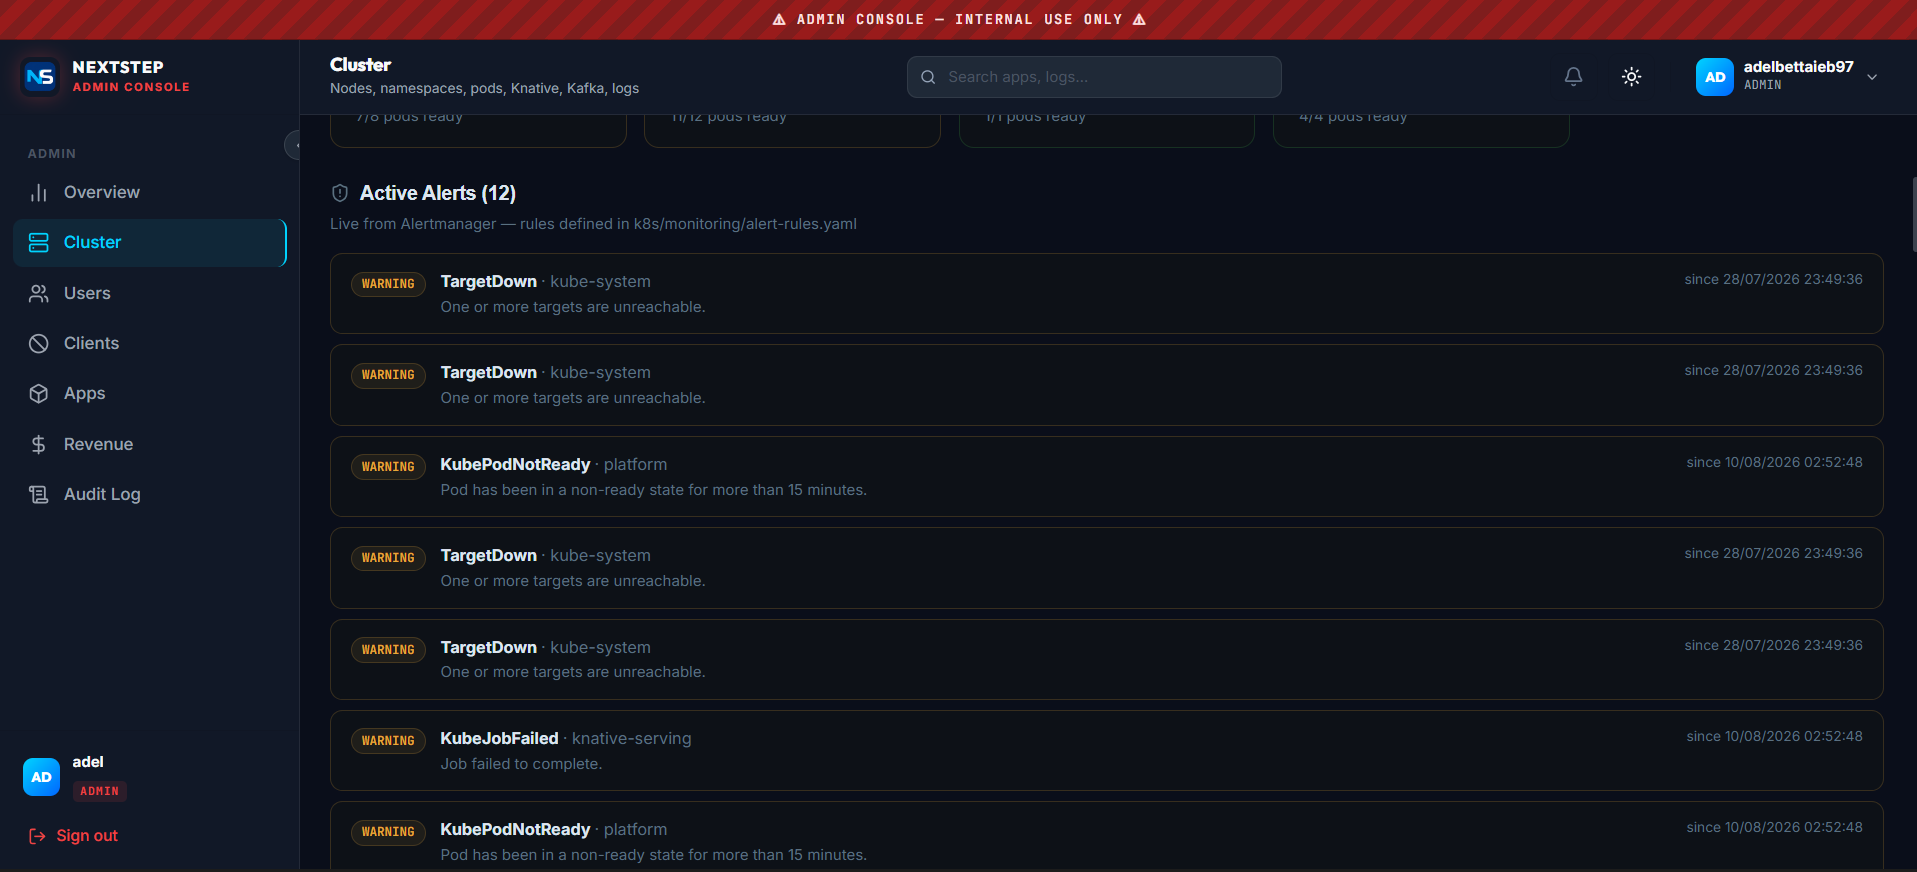
\includegraphics[width=0.9\textwidth]{image/Interface des alertes et événements du clust.png}
    \caption{Interface des alertes et événements du cluster}
    \label{fig:capture-alerts}
\end{figure}

\subsection{Conclusion}

Ce sprint clôt la Release 2 avec une supervision technique complète du cluster côté ADMIN, et une transparence de disponibilité offerte au public. La plateforme dispose désormais de l'ensemble des capacités de gestion applicative, de facturation et de supervision nécessaires à son exploitation par l'équipe de NextStep IT.

\section{Conclusion}

La Release 2 a complété la plateforme du point de vue de son exploitant : une facturation à l'usage mesurée automatiquement et réglable en ligne, une gouvernance des comptes clients tracée par un journal d'audit, et une supervision du cluster doublée d'une page de statut public. Comme pour la Release 1, plusieurs anomalies concrètes ont été identifiées et corrigées, et certaines limites ont été sciemment reportées, dans un contexte de ressources et de délai contraints, plutôt que dissimulées.
